
%%% Folie 1 %%%
  \begin{frame}
    \frametitle{Alternativen}
    \begin{itemize}
      \item Betriebssystem
      \item Messenger
      \item Google Alternativen
    \end{itemize}
  \end{frame}
  
%%% Folie 2 %%%
  \begin{frame}
    \frametitle{Betriebssystem}
    \textbf{Linux}
    \begin{itemize}
      \item Open Source \& Frei
      \item hohe Anpassbarkeit
      \item Paketverwaltung
      \item Auswahl an Distributionen \& Desktopumgebungen
    \end{itemize}
  \end{frame}
  
%%% Folie 3 %%%
  \begin{frame}
    \frametitle{Vergleich Messenger}
    \begin{tabular}{cccccc}
      \hline
      & Whatsapp & Threema & Telegram & Signal & Jabber \\
      \hline
      Verschlüsselung & \cellcolor{green} & \cellcolor{yellow} & \cellcolor{orange} & \cellcolor{green} & \cellcolor{green} \\
      \hline
      Vertrauensw. & \cellcolor{red} & \cellcolor{yellow} & \cellcolor{orange} & \cellcolor{green} &       \cellcolor{green} \\
      \hline
      Dezentr. & \cellcolor{red} & \cellcolor{red} & \cellcolor{red} & \cellcolor{orange} & \cellcolor{green} \\
      \hline
      Open Source & \cellcolor{red} & \cellcolor{orange} & \cellcolor{yellow} & \cellcolor{green} & \cellcolor{green} \\
      \hline
      Mobileignung & \cellcolor{green} & \cellcolor{green} & \cellcolor{green} & \cellcolor{green} & \cellcolor{green} \\
      \hline
    \end{tabular}
  \end{frame}

%%% Folie 4 %%%
  \begin{frame}{Owncloud}
    \begin{columns}
      \column{4cm}
      \footnotesize
Plattformübergreifende Synchronisierung von Dateien, Dokumenten, Kalendern, Kontakten, Notizen und News.
      \column{6cm}
      \begin{center}
        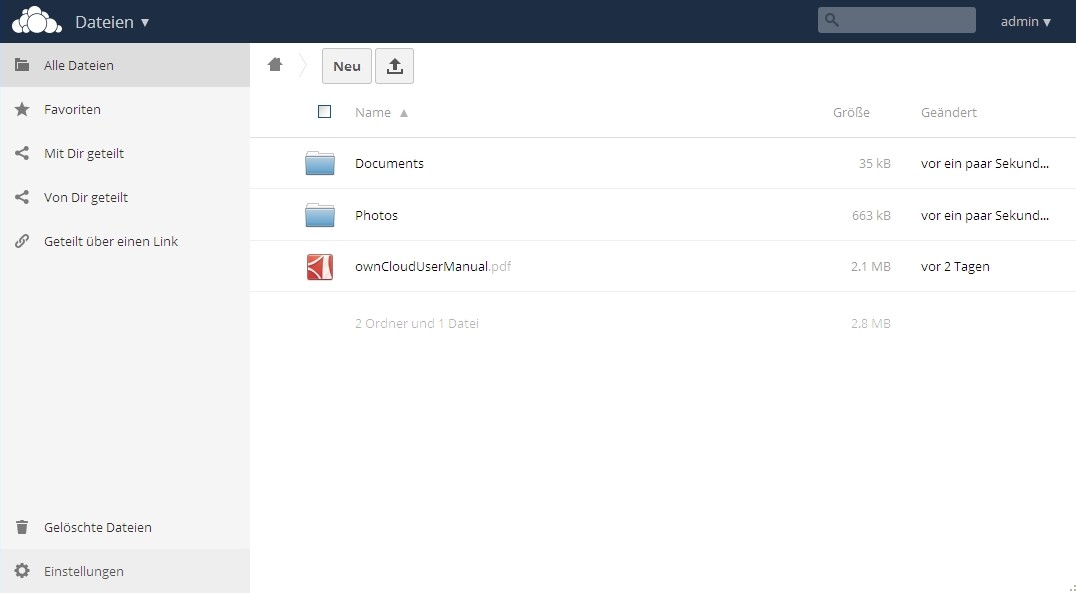
\includegraphics[width=6cm]{img/owncloud-screenshot.jpg}
        \par
      \end{center}
    \end{columns}
  \end{frame}

%%% Folie 5 %%%
  \begin{frame}{Owncloud als Ersatz für Dropbox}
    \begin{center}
      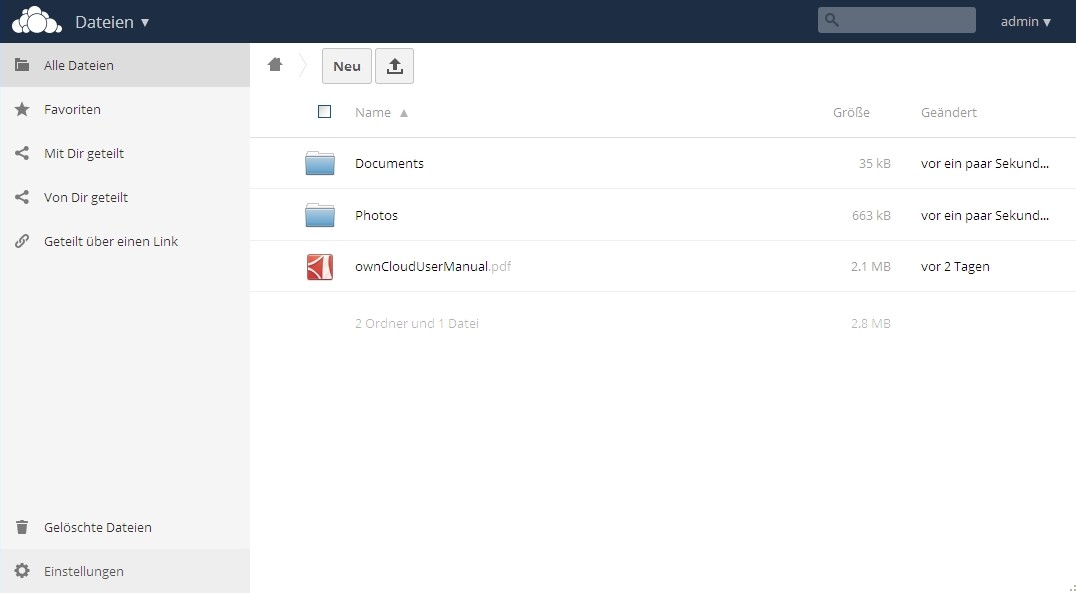
\includegraphics[width=9cm]{img/owncloud-screenshot.jpg}
    \end{center}
  \end{frame}

%%% Folie 6 %%%
  \begin{frame}{Owncloud als Ersatz für Google/Apple-Sync}
    \begin{center}
      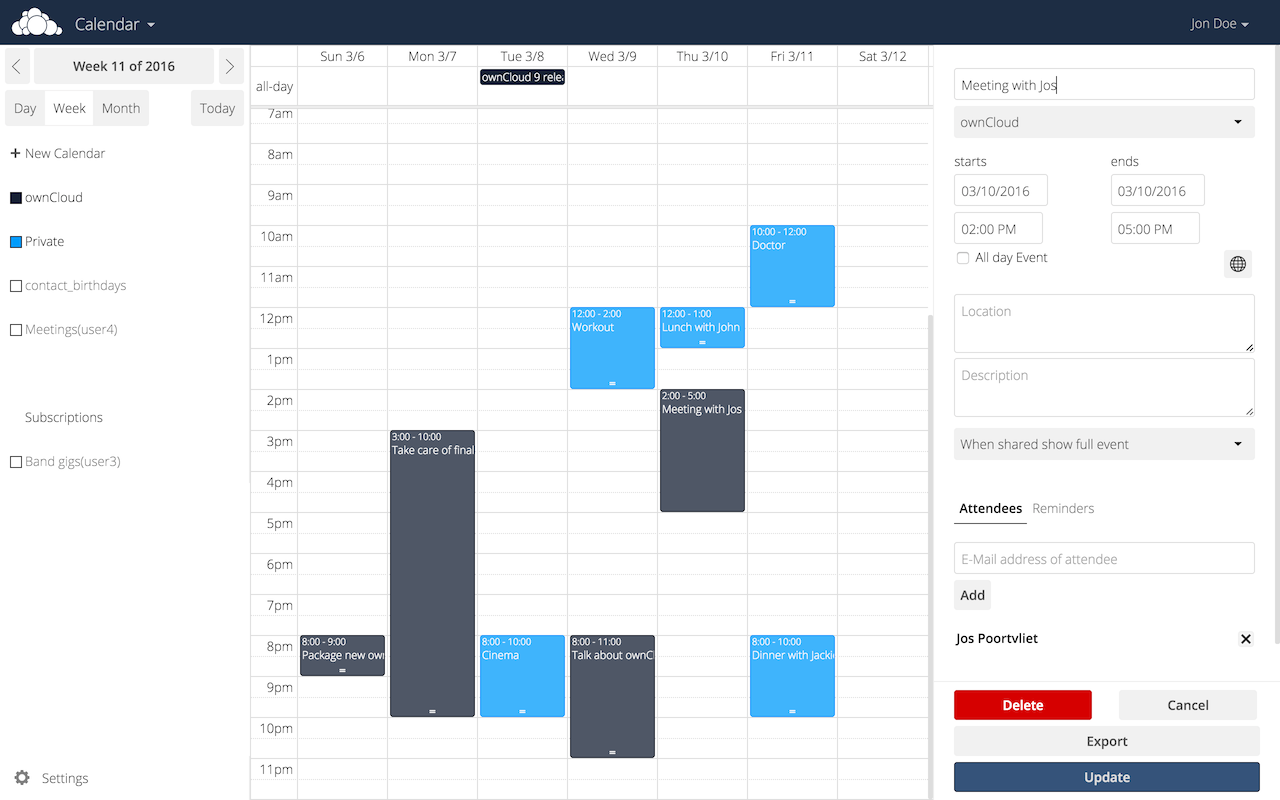
\includegraphics[width=9cm]{img/owncloud-calendar.png}
    \end{center}
  \end{frame}

%%% Folie 7 %%%
  \begin{frame}{Owncloud als Ersatz für Google/Apple-Sync}
    \begin{center}
      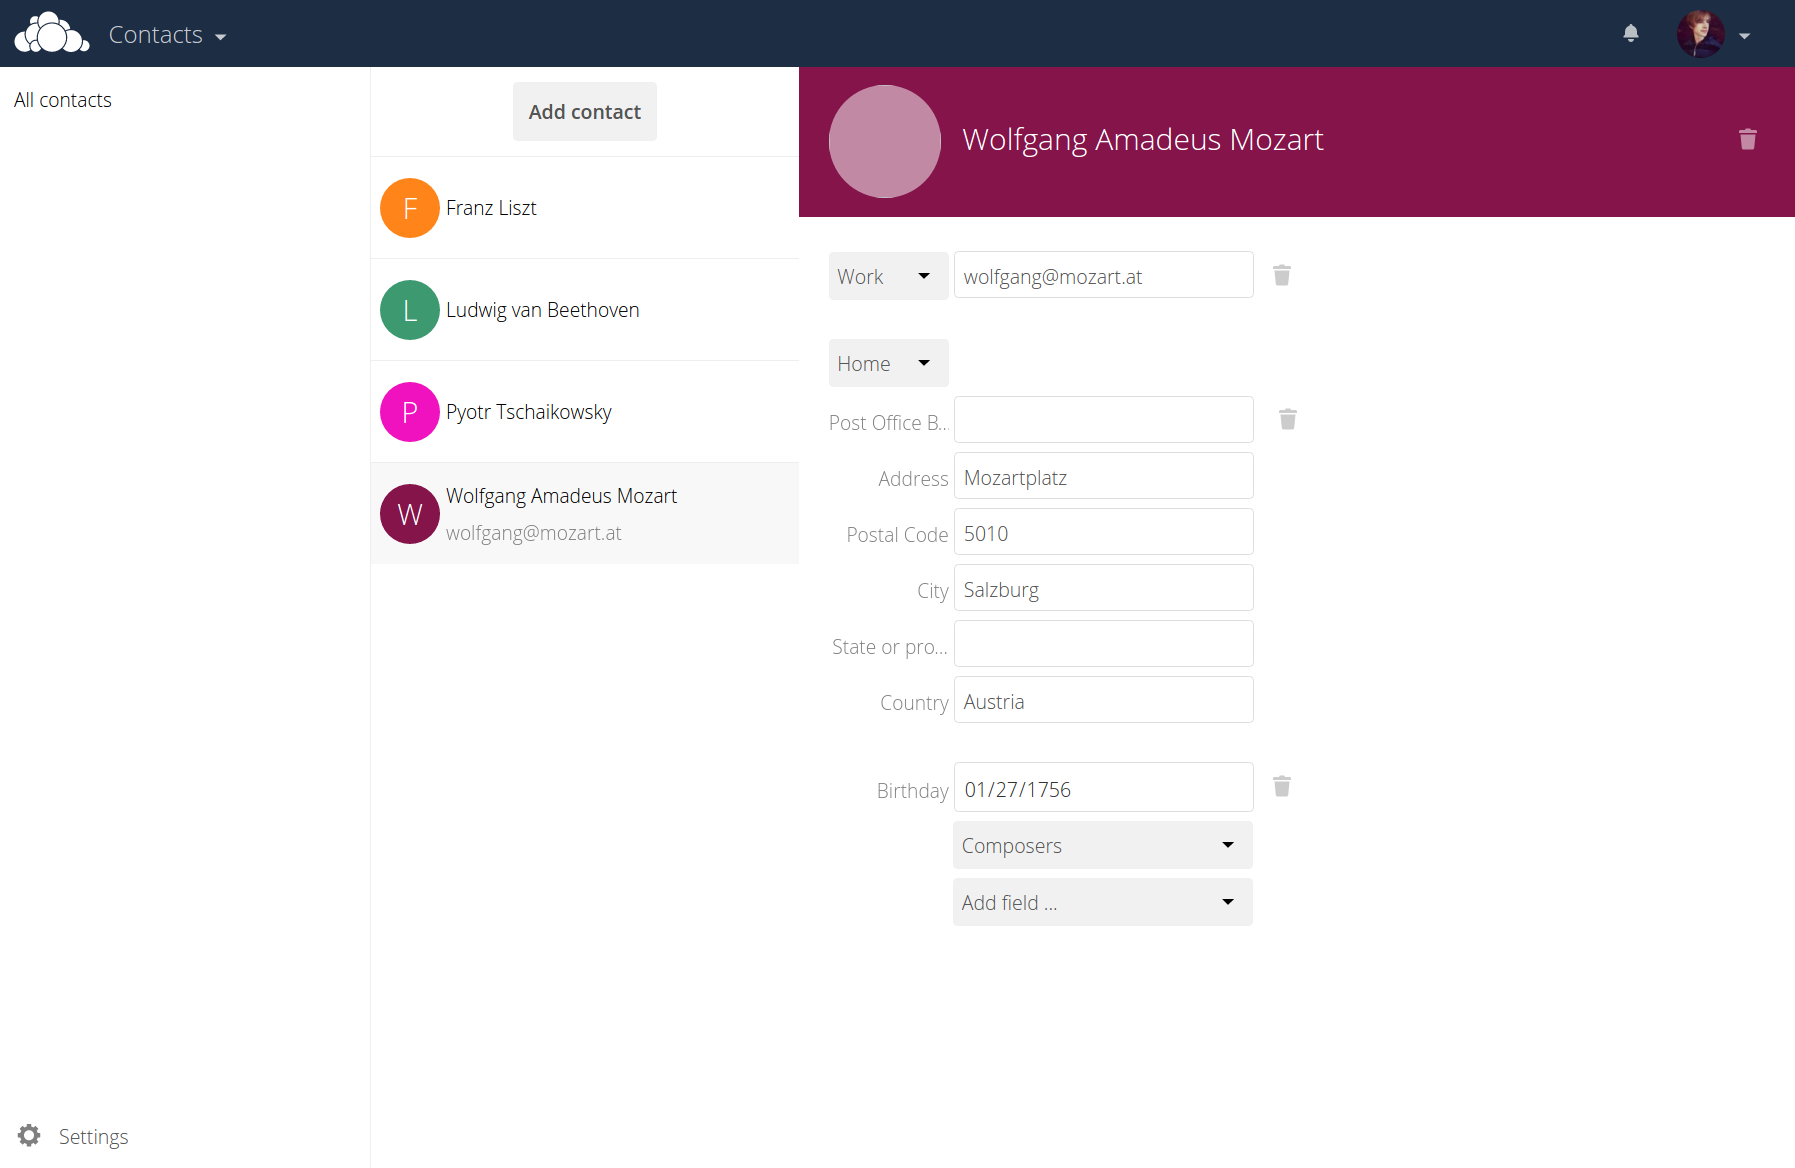
\includegraphics[width=9cm]{img/owncloud-contacts.png}
    \end{center}
  \end{frame}

%%% Folie 8 %%%
  \begin{frame}{Owncloud als Ersatz für Google Docs}
    \begin{center}
      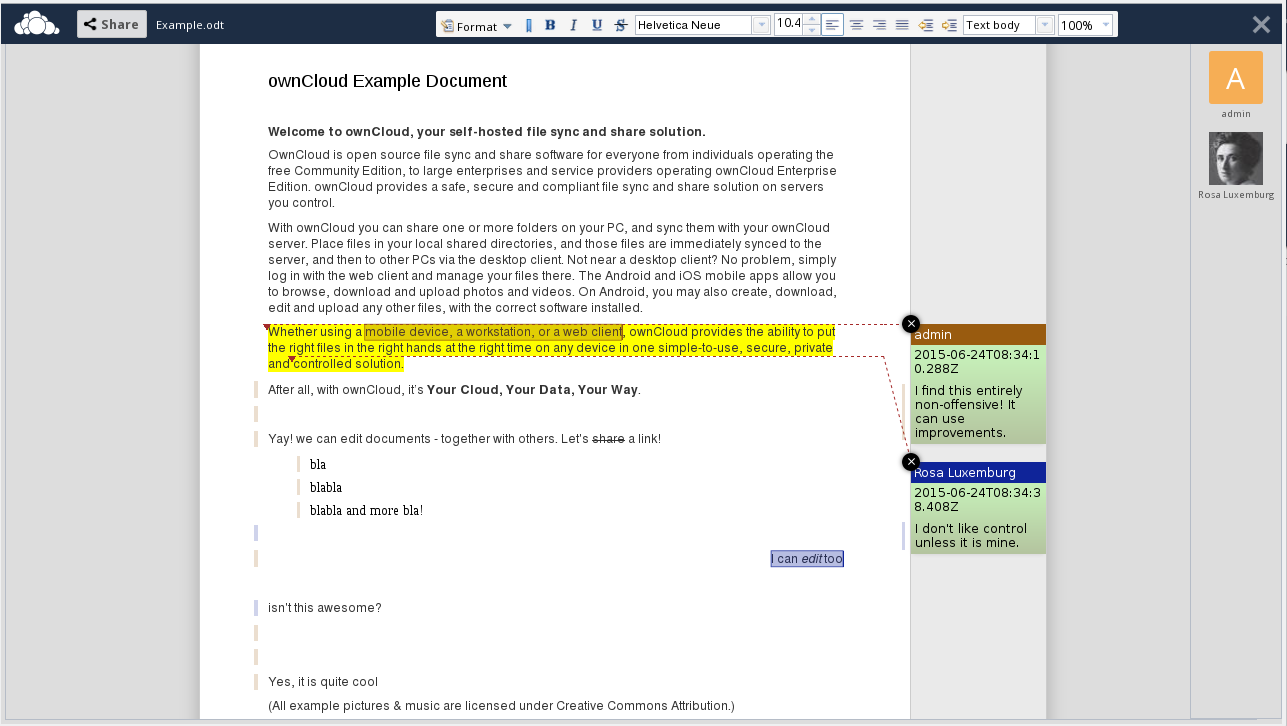
\includegraphics[width=9cm]{img/owncloud-documents.png}
    \end{center}
  \end{frame}

%%% Folie 9 %%%
  \begin{frame}
    \begin{columns}
      \column{6.5cm}
      \textbf{F-Droid}\\
      Android-Appstore für freie Software
      \vspace{0.5cm}
      \textbf{iOS Open Source Apps}\\
      
\includegraphics{img/fdroid.png}
      \column{5cm}
      \begin{center}
        
\includegraphics[width=2cm]{img/F-Droid_Logo_2.pdf}
        \par\end{center}
        \begin{center}
          \par
        \end{center}
    \end{columns}
  \end{frame}
  
%%% Folie 10 %%%
  \begin{frame}
    \frametitle{Alternative Suchmaschinen}
    \begin{columns}
        \begin{column}{5cm}
            \begin{center}
                    \begin{itemize}
                            \item Startpage
                            \vspace{2cm}
                            \item DuckDuckGo
                    \end{itemize}
            \end{center}
        \end{column}
        \begin{column}{5cm}
            \begin{center}
                
\includegraphics[width=0.5\textwidth]{img/startp_logo.png}
                \vspace{1cm}
                
\includegraphics[width=0.8\textwidth]{img/duckduckgo.png}
            \end{center}
        \end{column}
    \end{columns}
  \end{frame}
